\documentclass[lang=en, column=onecolumn, mathfont=times]{spArticle}
\spTitle{Group-Theoretical Analysis of Raman Spectra}
\spAuthor{Haixuan Lin: 23307110267}
\spAffiliation{Department of Physics, Fudan University}
\spDate{2025-12-24}
\spAbstract{
This paper systematically introduces the symmetry analysis of molecular vibrational modes in Raman spectroscopy from the perspective of group theory and molecular point group representation theory.
Building on a review of the physical mechanism of Raman scattering and its selection rules, we derive a general construction formula for the representation of molecular normal modes using the action of molecular point groups on the atomic space, configuration space, and the spaces of overall translation and rotation.
As a concrete example, the vibrational modes of the tetrahedral molecule $\ce{CCl4}$ are analyzed in detail: the irreducible decomposition of its representation is carried out in full, and the degeneracy of each vibrational mode together with its Raman and infrared activity is discussed with reference to the character table.
Furthermore, through a discussion of polarization experiments, we explain the group-theoretical origin of the disappearance of the $A_1$ mode peak under specific polarization conditions.
This paper aims to demonstrate the intuitive power and effectiveness of group-theoretical methods in molecular spectral analysis, providing a clear theoretical framework for understanding the connection between symmetry and experimental phenomena in Raman spectroscopy.
}

\usepackage{tikz-feynman}
\tikzfeynmanset{compat=1.1.0}

\newtheorem{theorem}{Theorem}

\begin{document}
\section{Motivation for Group-Theoretical Analysis}

In physics, symmetry implies conservation laws---its importance speaks for itself---and group theory provides a rigorous algebraic language for characterizing symmetry itself, making its introduction into physical research entirely natural. Today, group theory is widely applied across many branches of physics: condensed matter physics (the relationship between the symmetry of material structure and physical properties), modern theoretical physics (deriving physical laws purely from symmetry), and spectroscopy, which we shall discuss here. In a word, symmetry yields inequivalent irreducible eigenstates, which in turn give rise to spectral features.

In 1928, the Indian physicist C.~V.~Raman first observed scattered spectral lines with a shifted frequency in liquids~\cite{RamanKrishnan1928Nature}, for which he was awarded the Nobel Prize in Physics in 1930. At the time, techniques for resolving molecular structure were not yet mature, meaning that molecular configurations could not easily be determined. However, quantum mechanics tells us that Raman spectra are entirely determined by the vibrational characteristics of a molecule, and that the molecular configuration is an important cause of those characteristics; thus, inferring molecular configuration from Raman spectra was at the time an inverse problem in mathematical physics.

The present work, however, assumes that the configuration of the molecule of interest is already known, and applies group theory to analyze its spectrum---that is, it addresses the forward problem in mathematical physics. Although the forward problem is far less difficult than the inverse problem, it is highly instructive and directly connects theory to experiment, thereby deepening one's understanding of the physical phenomena.


\section{Methodology}

As shown below is a schematic of the Raman effect. It should be noted that the underlying process involves phonon resonance transitions rather than electronic ones. Because the molecule vibrates, the electronic energy levels of a polyatomic system split into multiple vibrational levels. On the electronic ground state, there exist many vibrational levels (phonon ground state, phonon excited states).

% \begin{figure}[H]
%     \centering
%     \begin{minipage}[c]{0.45\textwidth}
%         \centering
%         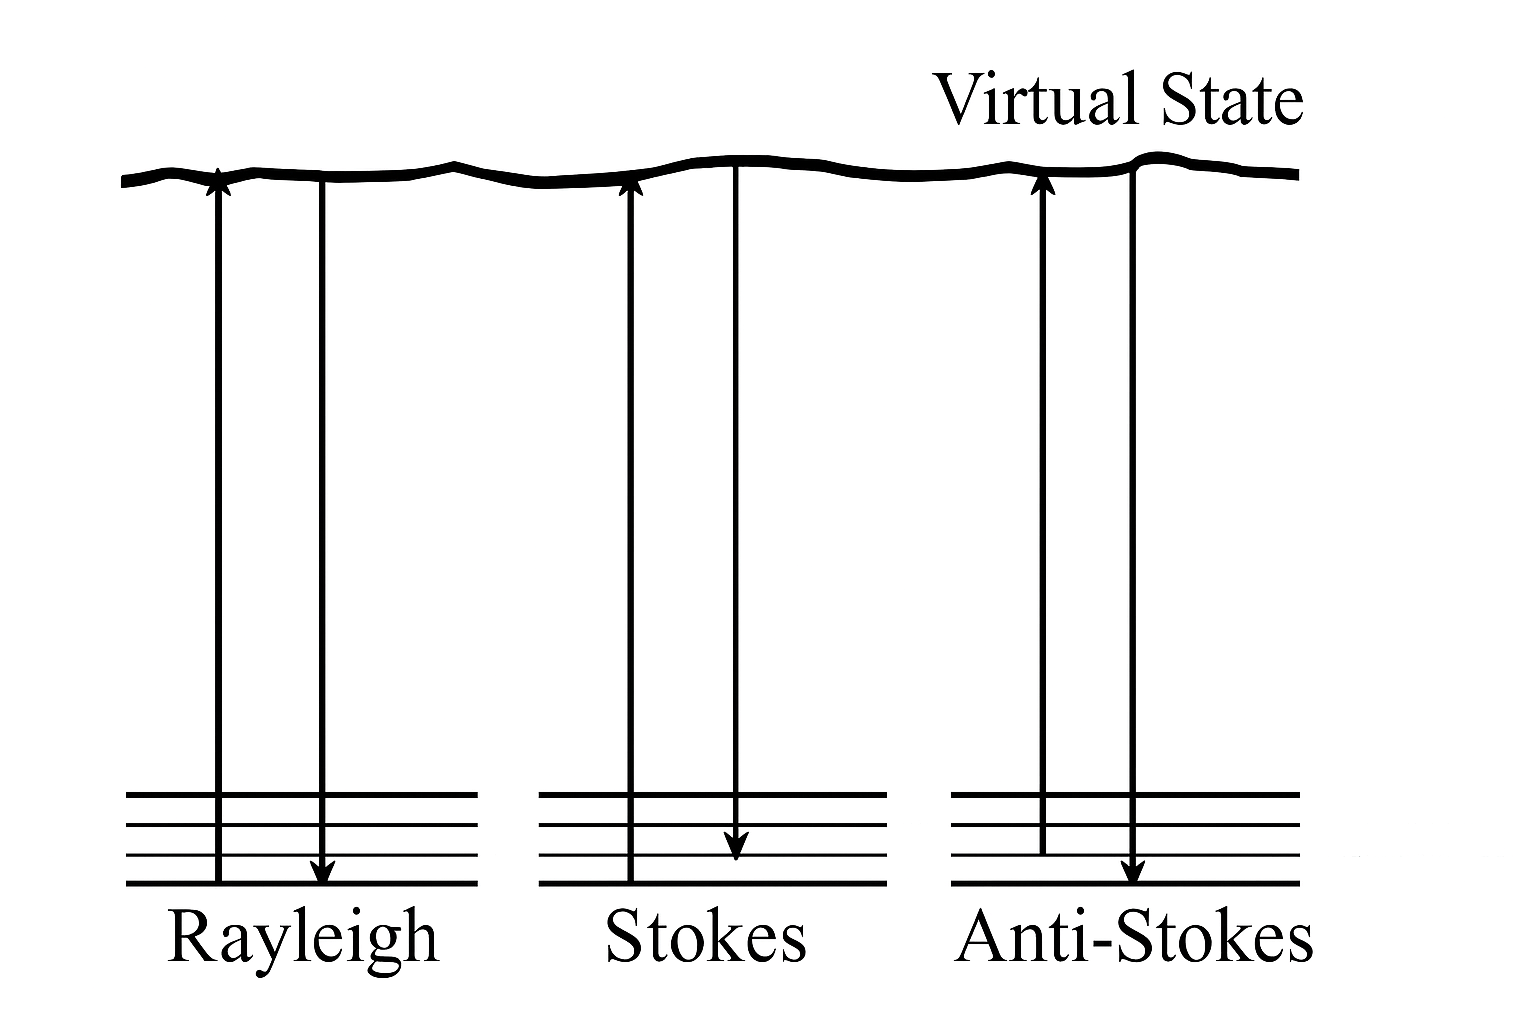
\includegraphics[width=\linewidth]{1.png}
%     \end{minipage}
%     \hfill
%     \begin{minipage}[c]{0.45\textwidth}
%         \centering
%         \feynmandiagram [horizontal=a to b] {
%               i1 [particle=$\gamma$]
%                   -- [fermion, very thick] a
%                   -- [fermion, opacity=0.45] i2 [particle=$\gamma \mp \Delta E$], 
        
%               a -- [red, photon, 
%                     edge label=$\pm \Delta E$, 
%                     momentum'={[arrow style=red]$\mathbf{k}$}] b, 
        
%               f1 [particle=$\mathrm{phonon}$]
%                   -- [fermion, opacity=0.45] b
%                   -- [fermion, very thick] f2 [particle=$\mathrm{phonon}\pm \Delta E$], 
%           };
%     \end{minipage}
%     \caption{Left: virtual excited state in the Raman effect; Right: Feynman diagram for (anti-)Stokes scattering}
% \end{figure}

The Raman scattering process involves a beam of light incident on a sample. Since photons are electromagnetic fields, they induce polarization in the sample molecules. In Placzek's theory, this polarization is described as a virtual absorption, in which the electron transitions from the ground state to a virtual excited state~\cite{Placzek1934Handbuch}.

For inelastic scattering:
\begin{itemize}
    \item Stokes: the initial state consists of the electronic ground state and the phonon ground state. During scattering, the photon loses energy, corresponding to a return to the electronic ground state and a phonon excited state; the photon energy is transferred to the phonon.
    \item Anti-Stokes: the initial state consists of the electronic ground state and a phonon excited state. The system returns to the electronic ground state and the phonon ground state; the phonon energy is transferred to the photon.
\end{itemize}

Where do the discrete phonon energy levels come from? We know that phonons have modes, and these modes originate from inequivalent irreducible normal modes. Treating the chemical bonds as providing first-order force constants while viewing higher-order forces as nonlinear perturbations (which can account for some slight peak splitting), i.e.\ modeling chemical bonds as springs, the Hamiltonian in the normal coordinates of the entire molecular system,
\begin{equation}
    H=\sum_{i=1}^N{\left( \frac{\boldsymbol{p}_{i}^{2}}{2m_i}+\frac{1}{2}m_i\omega _i\boldsymbol{q}_{i}^{2} \right)}
\end{equation}
is diagonal, with each diagonal element corresponding to one normal mode. Some normal modes are, however, equivalent: by ``equivalent'' we mean that they can be related to one another by a symmetry operation furnished by the molecular point group. Physically, such modes are said to be necessarily degenerate; symmetry protects them from being distinguished unless a perturbation that lowers the symmetry is applied.

% \begin{figure}[H]
%     \centering
    
%     \setchemfig{arrow length=70mm}
%     \setchemfig{compound sep=20em}
    
%     \schemestart
%     \chemfig{
%         C
%         (-[:90]Cl)
%         (<[:250, 1.1]Cl)
%         (-[:340]Cl)
%         (<:[:200, 1.1]Cl)
%     }
%     \chemmove{
%         \draw[<->, >=stealth, very thick] (-1.1, 0.2) -- (-1.1, 1) node[left, midway, xshift=4.5em, yshift=1em] {$\text{vibration}$};
%         }
%     \arrow{<->[$\text{the two modes can be related by a rotation}$][$\text{necessary degeneracy}$]}
%     \chemfig{
%         C
%         (-[:90]Cl)
%         (<[:250, 1.1]Cl)
%         (-[:340]Cl)
%         (<:[:200, 1.1]Cl)
%     }
%     \chemmove{
%         \draw[<->, >=stealth, very thick] (-1.2, 0.3) -- ++(340:0.8) node[left, midway, xshift=3.5em, yshift=1em] {$\text{vibration}$};
%         }
%     \schemestop
    
%     \caption{Schematic illustration of necessary degeneracy of vibrational modes in CCl$_4$}
% \end{figure}

Our goal is to find all inequivalent irreducible normal modes of a given molecule. The following theorem provides the means:
\begin{theorem}
    \label{thm}
    Define the following linear spaces:
    \begin{itemize}
        \item $V^{\mathrm{a.s.}}=\mathrm{span}\left\{X_i\right\}_{i=1}^N$ is a linear space over $\mathbb{C}$, where $X_i$ denotes an atom and $N$ is the total number of atoms in the molecule;
        \item $V_{\mathrm{vec}}=\left\{\left(x, y, z\right)\right\}$ is the linear space of configuration vectors;
        \item $V_{\mathrm{trans}}$ is the space spanned by vectors describing translation;
        \item $V_{\mathrm{rot}}$ is the space spanned by vectors describing rotation.
    \end{itemize}
    Let $\Gamma ^{\mathrm{a.s.}}, \Gamma _{\mathrm{vec}}, \Gamma _{\mathrm{trans}}, \Gamma _{\mathrm{rot}}$ denote the representations of the molecular point group on these spaces, respectively. Then the representation of molecular vibrations is
    \begin{equation}
        \Gamma _{\mathrm{mol}.\mathrm{vib}.}=\left( \Gamma ^{\mathrm{a}.\mathrm{s}.}\otimes \Gamma _{\mathrm{vec}} \right) \ominus \Gamma _{\mathrm{trans}}\ominus \Gamma _{\mathrm{rot}}.
    \end{equation}
\end{theorem}
The proof is evident from the physical interpretation: the representation spanned by molecular vibrational modes should equal the representation spanned by all degrees of freedom, minus those spanned by overall translation and overall rotation. The total degrees of freedom of the molecule, in turn, are given by the tensor product of the atomic species and the three translational degrees of freedom in Euclidean space $E^3$.

The rigorous proof is as follows. Let $\Gamma_{3N}$ be the representation on the configuration space in which all atoms move freely. We wish to show that $\Gamma_{3N} \simeq \Gamma^{\mathrm{a.s.}} \otimes \Gamma_{\mathrm{vec}}$, or equivalently, that $V_{3N} \simeq V^{\mathrm{a.s.}} \otimes V_{\mathrm{vec}}$. In terms of a commutative diagram:
\[
\begin{tikzcd}[
        background color=white,      % 整个图背景（可选）
        every label/.append style={  % 所有箭头标签样式追加
            % text=white,                % 标签文字白色
            % fill=white,                % 标签背景黑色
            inner sep=2pt              % 标签内间距
        }
        ]
        \Gamma_{3N} \arrow[r, "\simeq" description, no head, phantom]
            & \Gamma^{\mathrm{a.s.}} \arrow[r, "\otimes" description, no head, phantom] & \Gamma_{\mathrm{vec}} \\
        V_{3N} \arrow[u] \arrow[r, "\simeq" description, no head, phantom]
            & V^{\mathrm{a.s.}} \arrow[u] \arrow[r, "\otimes" description, no head, phantom] & V_{\mathrm{vec}} \arrow[u]
        \end{tikzcd}
\]
For any atom $X_i$ and any coordinate $\mu$, with $i=1,\cdots, N$ and $\mu=x,y,z$, one always has
\begin{equation}
    \left| X_i\mu \right> =\left| X_i \right> \otimes \left| \mu \right>,
\end{equation}
where the latter two factors are precisely bases of $V^{\mathrm{a.s.}}$ and $V_{\mathrm{vec}}$, respectively. This completes the proof.

The following expression provides an interpretation of the theorem from the perspective of dimensions:
\vspace{2em}
\begin{equation}
    \tikzmarknode{1}{\hlmath{gray}{\Gamma _{\mathrm{mol}.\mathrm{vib}.}}}
    =
    \left( \tikzmarknode{2}{\hlmath{gray}{\Gamma ^{\mathrm{a}.\mathrm{s}.}}}
    \otimes
    \tikzmarknode{3}{\hlmath{gray}{\Gamma _{\mathrm{vec}} }}\right)
    \ominus
    \tikzmarknode{4}{\hlmath{gray}{\Gamma _{\mathrm{trans}}}}
    \ominus
    \tikzmarknode{5}{\hlmath{gray}{\Gamma _{\mathrm{rot}}}}.
\end{equation}
\vspace{2em}
\begin{tikzpicture}[overlay, remember picture, >=stealth, nodes={align=left, inner ysep=2pt}, <-]
    \path (1.south) ++ (0, -0.8em) node[anchor=north east, color=gray!67] (1 node){$\mathrm{dim}=3N-6$};
    \draw [color=gray!57](1.south) |- ([xshift=-0.3ex, color=gray]1 node.south west);
\end{tikzpicture}
\begin{tikzpicture}[overlay, remember picture, >=stealth, nodes={align=left, inner ysep=2pt}, <-]
    \path (1.north) ++ (0, +1em) node[anchor=south west, color=gray!67] (1 node){total d.o.f.\ ($3N$) $-$ overall translation ($3$) $-$ overall rotation ($3$)};
    \draw [color=gray!57](1.north) |- ([xshift=-0.3ex, color=gray]1 node.south east);
\end{tikzpicture}
\begin{tikzpicture}[overlay, remember picture, >=stealth, nodes={align=left, inner ysep=1pt}, <-]
\node[anchor=north, color=gray!67, yshift=-2em] (jtext) at ($(2.south)!0.5!(3.south)$) {$\mathrm{dim}=N\times 3$};
\draw[<->, color=gray!57] (2.south) |- (jtext.north) -| (3.south);
\end{tikzpicture}
\begin{tikzpicture}[overlay, remember picture, >=stealth, nodes={align=left, inner ysep=2pt}, <-]
    \path (4.south) ++ (0, -1.8em) node[anchor=north west, color=gray!67] (4 node){$\mathrm{dim}=3$};
    \draw [color=gray!57](4.south) |- ([xshift=+0.3ex, color=gray]4 node.south east);
\end{tikzpicture}
\begin{tikzpicture}[overlay, remember picture, >=stealth, nodes={align=left, inner ysep=2pt}, <-]
    \path (5.south) ++ (0, -0.5em) node[anchor=north west, color=gray!67] (5 node){$\mathrm{dim}=3$};
    \draw [color=gray!57](5.south) |- ([xshift=+0.3ex, color=gray]5 node.south east);
\end{tikzpicture}

In principle, this theorem can be used to analyze the normal modes of any molecule. For molecules with low symmetry, however, few point group operations are available, and nearly all of the resolved modes turn out to be one-dimensional. Physically, this can be understood as follows: because the molecular symmetry is low, any two vibrational modes can easily be distinguished.


\section{An Illustrative Application: The Spectrum of \texorpdfstring{$\ce{CCl4}$}{CCl4}}

\subsection{Finding the Inequivalent Irreducible Normal Modes}
\label{subsec}

The molecular structure of $\ce{CCl4}$ is shown below. The central carbon atom is $\mathrm{sp}^3$ hybridized, giving the molecule an overall tetrahedral geometry that belongs to the $T_\mathrm{d}$ point group, which has order 24.

% \begin{figure}[H]
%     \centering
%     \chemfig{
%         C
%         (-[:90]Cl)
%         (<[:250, 1.1]Cl)
%         (-[:340]Cl)
%         (<:[:200, 1.1]Cl)
%     }
%     \chemmove{
%     \draw[<->, >=stealth] (-0.7, 0) arc[start angle=0, end angle=70, radius=0.8cm]
%         node[right, xshift=5pt, yshift=-2pt] {\small $109.5^\circ$};
%     }
%     \caption{Structural formula of \texorpdfstring{$\ce{CCl_4}$}{CCl4}}
% \end{figure}

By \textbf{Burnside's theorem}, the 24-dimensional group algebra contains all irreducible representations in its left regular representation, and the multiplicity of each irreducible representation $\Gamma_i$ equals $\mathrm{dim}\,\Gamma_i$:
\begin{equation}
    \mathbb{C} \left[ T_{\mathrm{d}} \right] \simeq \bigotimes_i{\left( \mathrm{dim}\, \Gamma _i \right) \Gamma _i}.
\end{equation}
Taking the modulus on both sides gives the integer decomposition
\begin{equation}
    24 = 1^2 + 1^2 + 2^2 + 3^2 + 3^2,
\end{equation}
showing that $T_\mathrm{d}$ has exactly 5 inequivalent irreducible representations (one of which is the trivial representation). The character table is:
\begin{table}[H]
    \centering
    \renewcommand{\arraystretch}{1.2}
    \begin{tabular}{|c|c|c|c|c|c|c|c|}
        \hline
        $T_d$ & $E$ & $8C_3$ & $3C_2$ & $6S_4$ & $6\sigma_d$
            & \text{linear functions}
            & \text{quadratic functions} \\
        \hline
        $A_1$ & +1 & +1 & +1 & +1 & +1
            & --
            & $x^2+y^2+z^2$ \\
        \hline
        $A_2$ & +1 & +1 & +1 & -1 & -1
            & --
            & -- \\
        \hline
        $E$   & +2 & -1 & +2 & 0  & 0
            & --
            & $(2z^2-x^2-y^2, \;x^2-y^2)$ \\
        \hline
        $T_1$ & +3 & 0  & -1 & +1 & -1
            & $(R_x, R_y, R_z)$
            & -- \\
        \hline
        $T_2$ & +3 & 0  & -1 & -1 & +1
            & $(x, y, z)$
            & $(xy, xz, yz)$ \\
        \hline
        \multicolumn{8}{c}{} \\
        \hline
        $\Gamma ^{\mathrm{a}.\mathrm{s}.}_{4\ce{Cl}}$ & 4 & 1 & 0 & 2 & 0 & \multicolumn{1}{c}{$\Rightarrow A_1\oplus T_2$} &   \\
        \hline
    \end{tabular}
    \caption{Character table of the $T_\mathrm{d}$ group.}
    \label{table}
\end{table}

We first compute $\Gamma ^{\mathrm{a.s.}}$. Since the symmetry permutations of the molecular point group act only among chemically equivalent atoms, the following decomposition holds:
\begin{align*}
        &\underbrace{
            \mathrm{span}\left\{
            \chemfig{
                C
                (-[:90]Cl)
                (<[:250, 1.1]Cl)
                (-[:340]Cl)
                (<:[:200, 1.1]Cl)
            }
        \right\}
        }{\tikzmarknode{a}{}}
        &{\hspace{-1em}\scalebox{2}{$\simeq$}}\hphantom{-}
        &\underbrace{\mathrm{span}\left\{
            \chemfig{
                \phantom{C}
                (-[:90]Cl)
                (<[:250, 1.1]Cl)
                (-[:340]Cl)
                (<:[:200, 1.1]Cl)
            }
        \right\}
        }{\tikzmarknode{b}{}}
        &\hspace{-1em}\bigoplus\hspace{1em}
        &\underbrace{\mathrm{span}\left\{
            \hphantom{\scalebox{0.3}{%
            \chemfig{
                C
                (-[:90]Cl)
                (<[:250, 1.1]Cl)
                (-[:340]Cl)
                (<:[:200, 1.1]Cl)
            }
            }}
            \vphantom{\chemfig{
                C
                (-[:90]Cl)
                (<[:250, 1.1]Cl)
                (-[:340]Cl)
                (<:[:200, 1.1]Cl)
            }}
            \ce{C}
            \hphantom{\scalebox{0.3}{%
            \chemfig{
                C
                (-[:90]Cl)
                (<[:250, 1.1]Cl)
                (-[:340]Cl)
                (<:[:200, 1.1]Cl)
            }
            }}
        \right\}, 
        }{\tikzmarknode{c}{}}
        \\
        &\hspace{5em}\Gamma ^{\mathrm{a}.\mathrm{s}.}
        &\phantom{\simeq}
        &\hspace{5em}\Gamma ^{\mathrm{a}.\mathrm{s}.}_{4\ce{Cl}}
        &\phantom{\oplus}
        &\hspace{4em}\Gamma ^{\mathrm{a}.\mathrm{s}.}_{\ce{C}}.
    \end{align*}
    
The linear space corresponding to the carbon atom is one-dimensional, so it must carry the trivial representation:
\begin{equation}
    \Gamma ^{\mathrm{a}.\mathrm{s}.}_{\ce{C}}\simeq A_1.
    \label{eq: 6}
\end{equation}

We now compute $\Gamma ^{\mathrm{a}.\mathrm{s}.}_{4\ce{Cl}}$. We consider the representation of the four chlorine atoms under symmetry operations that preserve the configuration. Since any permutation of two chlorine atoms leaves the system invariant,
$$
T_{\mathrm{d}}\simeq S_4\quad \left( \text{symmetric group on 4 elements} \right).
$$
The generators of $S_4$ are $(12)$ and $(1234)$, whose matrix representations are
$$
    \left( \begin{matrix}
    &		1&		&		\\
    1&		&		&		\\
    &		&		1&		\\
    &		&		&		1\\
\end{matrix} \right) , \qquad \left( \begin{matrix}
    &		&		&		1\\
    1&		&		&		\\
    &		1&		&		\\
    &		&		1&		\\
\end{matrix} \right).
$$
From these, one can compute the character of each conjugacy class of $T_\mathrm{d}$ in the linear space of the four chlorine atoms. Applying the \textbf{orthogonality and completeness theorem for characters}, we look up the table and decompose $\Gamma ^{\mathrm{a.s.}}_{4\ce{Cl}}$:
\begin{equation}
    \Gamma ^{\mathrm{a}.\mathrm{s}.}_{4\ce{Cl}}\simeq A_1\oplus T_2.
    \label{eq: 7}
\end{equation}

Combining \eqref{eq: 6} and \eqref{eq: 7}:
\begin{equation*}
    \Gamma ^{\mathrm{a}.\mathrm{s}.}\simeq
    \Gamma ^{\mathrm{a}.\mathrm{s}.}_{4\ce{Cl}}\oplus \Gamma ^{\mathrm{a}.\mathrm{s}.}_{\ce{C}}\simeq \left( A_1\oplus T_2 \right) \oplus A_1\simeq 2A_1\oplus T_2.
\end{equation*}
To find $\Gamma _{\mathrm{trans}}$ and $\Gamma _{\mathrm{rot}}$, we use the symmetrized basis functions of the irreducible representations. The symmetry of $\Gamma _{\mathrm{trans}}$ matches that of $\left(x, y, z\right)$, while $\Gamma _{\mathrm{rot}}$ matches $\left( R_x, R_y, R_z \right)$, the axial vectors represented by the angular momentum vector, so
\begin{equation}
    {\Gamma _{\mathrm{trans}}\simeq T_2}, \qquad {\Gamma _{\mathrm{rot}}\simeq T_1}.
    \label{eq: 8}
\end{equation}

Finally, applying Theorem~\ref{thm}:
$$
\begin{aligned}
    \Gamma _{\mathrm{mol}.\mathrm{vib}.}&=\left( \Gamma ^{\mathrm{a}.\mathrm{s}.}\otimes \Gamma _{\mathrm{vec}} \right) \ominus \Gamma _{\mathrm{trans}}\ominus \Gamma _{\mathrm{rot}}
    \\
    &=\left[ \left( 2A_1\oplus T_2 \right) \otimes T_2 \right] \ominus T_2\ominus T_1
    \\
    &=2\underset{A_1\otimes T_2}{\underbrace{T_2}}\oplus \underset{T_2\otimes T_2}{\underbrace{T_1\oplus T_2\oplus E\oplus A_1}}\ominus T_2\ominus T_1
    \\
    &=A_1\oplus E\oplus 2T_2.
\end{aligned}
$$
This is the irreducible decomposition of the normal-mode representation of $\ce{CCl4}$: there are four inequivalent irreducible modes, consisting of one $A_1$ mode, one $E$ mode, and two $T_2$ modes (both have $T_2$ symmetry, but they are not equivalent to each other).

Group theory cannot provide the eigenenergy of each mode; that requires quantum mechanics (and modern first-principles calculations can indeed compute Raman shifts with high accuracy). This is not the focus of the present paper. The figure below directly shows the mode assignment for each peak, using $\nu_i$ to label the different modes\footnote{Labeling modes by their representation alone cannot distinguish the two $T_2$ modes, so an additional notation is necessary.}:

% \begin{figure}[H]
%     \centering
%     \resizebox{0.85\linewidth}{!}{% This file was created by matlab2tikz.
%
%The latest updates can be retrieved from
%  http://www.mathworks.com/matlabcentral/fileexchange/22022-matlab2tikz-matlab2tikz
%where you can also make suggestions and rate matlab2tikz.
%
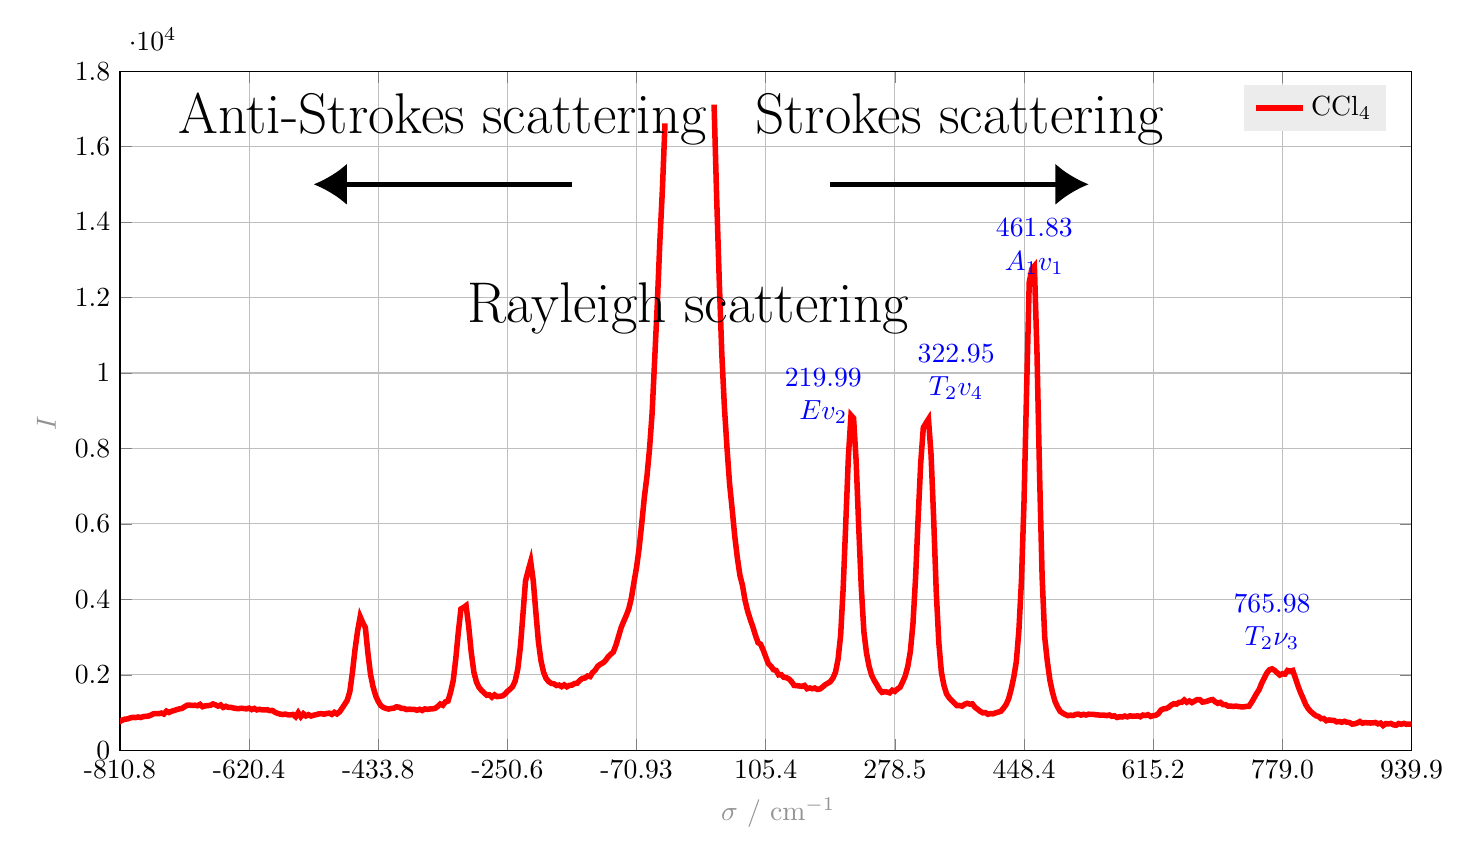
\begin{tikzpicture}

\begin{axis}[%
width=6.458in,
height=3.396in,
at={(1.083in,0.458in)},
scale only axis,
clip=true,
xmin=510,
xmax=560,
xtick={510,515,520,525,530,535,540,545,550,555,560},
xticklabels={{-810.8},{-620.4},{-433.8},{-250.6},{-70.93},{105.4},{278.5},{448.4},{615.2},{779.0},{939.9}},
xlabel style={font=\color{gray!85!white}},
xlabel={波数 $\sigma$ / $\mathrm{cm}^{-1}$},
ymin=0,
ymax=18000,
ylabel style={font=\color{gray!85!white}},
ylabel={$I$ 强度},
% axis background/.style={fill=},
xmajorgrids,
ymajorgrids,
legend style={legend cell align=left, align=left, draw=white!85!gray, fill=white!85!gray},
restrict y to domain=0:18000
]
\addplot [color=red, line width=2.0pt]
  table[row sep=crcr]{%
505	647.8\\
505.1	641\\
505.2	644.2\\
505.3	641\\
505.4	656.9\\
505.5	676.4\\
505.6	691.5\\
505.7	696.8\\
505.8	685.8\\
505.9	662.8\\
506	637.2\\
506.1	657\\
506.2	662.5\\
506.3	672\\
506.4	678.6\\
506.5	689.5\\
506.6	676.8\\
506.7	715.8\\
506.8	703.5\\
506.9	726.2\\
507	708.5\\
507.1	712.8\\
507.2	705.5\\
507.3	737.5\\
507.4	700.2\\
507.5	711.5\\
507.6	686.5\\
507.7	702\\
507.8	703.5\\
507.9	727.9\\
508	720.2\\
508.1	746.5\\
508.2	715.5\\
508.3	743.5\\
508.4	731\\
508.5	715.2\\
508.6	733.5\\
508.7	732.4\\
508.8	739\\
508.9	737.4\\
509	723.9\\
509.1	727.6\\
509.2	745.3\\
509.3	746.4\\
509.4	751.5\\
509.5	754.2\\
509.6	754\\
509.7	772.8\\
509.8	747.5\\
509.9	775.5\\
510	765.5\\
510.1	802.6\\
510.2	827.3\\
510.3	832.1\\
510.4	859\\
510.5	874.2\\
510.6	867.5\\
510.7	882.9\\
510.8	870.8\\
510.9	893.6\\
511	900.1\\
511.1	907.6\\
511.2	934.5\\
511.3	968.8\\
511.4	973.1\\
511.5	970.5\\
511.6	988\\
511.7	962\\
511.8	1039\\
511.9	1002.7\\
512	1036.5\\
512.1	1055.3\\
512.2	1079.9\\
512.3	1098.6\\
512.4	1109.5\\
512.5	1154.8\\
512.6	1194.3\\
512.7	1199\\
512.8	1189.5\\
512.9	1195.1\\
513	1182.7\\
513.1	1217.5\\
513.2	1156\\
513.3	1177.6\\
513.4	1185.2\\
513.5	1191.5\\
513.6	1229.2\\
513.7	1203.2\\
513.8	1171.2\\
513.9	1202.5\\
514	1137.5\\
514.1	1166.1\\
514.2	1138.2\\
514.3	1137.8\\
514.4	1120.4\\
514.5	1108.8\\
514.6	1105.2\\
514.7	1114.9\\
514.8	1107.5\\
514.9	1099.2\\
515	1117.6\\
515.1	1079.5\\
515.2	1108.8\\
515.3	1071\\
515.4	1087.1\\
515.5	1074.5\\
515.6	1069.5\\
515.7	1075.9\\
515.8	1052.5\\
515.9	1057.1\\
516	1010\\
516.1	980.5\\
516.2	960.4\\
516.3	949.1\\
516.4	960.3\\
516.5	942\\
516.6	940.2\\
516.7	950.4\\
516.8	890.5\\
516.9	997.5\\
517	891\\
517.1	969.7\\
517.2	911.5\\
517.3	944.5\\
517.4	909.9\\
517.5	931.1\\
517.6	944.8\\
517.7	966\\
517.8	972.4\\
517.9	957.4\\
518	975.5\\
518.1	985\\
518.2	952\\
518.3	1005.5\\
518.4	964.4\\
518.5	1017.1\\
518.6	1115.1\\
518.7	1221\\
518.8	1329.2\\
518.9	1556.8\\
519	2067.3\\
519.1	2671.2\\
519.2	3162.1\\
519.3	3541.2\\
519.4	3382\\
519.5	3252.7\\
519.6	2571.8\\
519.7	2013.3\\
519.8	1680.4\\
519.9	1445.8\\
520	1293.9\\
520.1	1183.9\\
520.2	1137.5\\
520.3	1109\\
520.4	1094.5\\
520.5	1110\\
520.6	1117.2\\
520.7	1153.1\\
520.8	1143.3\\
520.9	1110\\
521	1108\\
521.1	1080.5\\
521.2	1089.8\\
521.3	1086.4\\
521.4	1083\\
521.5	1062.3\\
521.6	1087.5\\
521.7	1056.7\\
521.8	1097.9\\
521.9	1085.5\\
522	1095.6\\
522.1	1099\\
522.2	1113.1\\
522.3	1161.6\\
522.4	1227.3\\
522.5	1194.5\\
522.6	1284.5\\
522.7	1307.2\\
522.8	1540.7\\
522.9	1842.8\\
523	2422\\
523.1	3138.2\\
523.2	3746.5\\
523.3	3784.5\\
523.4	3835.6\\
523.5	3286.9\\
523.6	2591.6\\
523.7	2079.2\\
523.8	1811.7\\
523.9	1667.8\\
524	1586.3\\
524.1	1521.4\\
524.2	1459.2\\
524.3	1469.5\\
524.4	1409.5\\
524.5	1469.5\\
524.6	1423.3\\
524.7	1432.5\\
524.8	1441.7\\
524.9	1487.2\\
525	1563\\
525.1	1618.1\\
525.2	1689.8\\
525.3	1837.5\\
525.4	2151.5\\
525.5	2727.2\\
525.6	3594.4\\
525.7	4485\\
525.8	4757.5\\
525.9	5001.7\\
526	4492.8\\
526.1	3665.7\\
526.2	2875.7\\
526.3	2370\\
526.4	2067.2\\
526.5	1901\\
526.6	1819.6\\
526.7	1773.7\\
526.8	1763.2\\
526.9	1718\\
527	1729.9\\
527.1	1689\\
527.2	1734.5\\
527.3	1683.5\\
527.4	1721.6\\
527.5	1729.5\\
527.6	1770.3\\
527.7	1780\\
527.8	1852.7\\
527.9	1906.3\\
528	1916.3\\
528.1	1969.5\\
528.2	1953.2\\
528.3	2063.2\\
528.4	2128.3\\
528.5	2231.9\\
528.6	2281\\
528.7	2317.9\\
528.8	2382.9\\
528.9	2480.3\\
529	2547\\
529.1	2605.4\\
529.2	2784.8\\
529.3	3014.7\\
529.4	3249.3\\
529.5	3416.8\\
529.6	3571.9\\
529.7	3752.1\\
529.8	4041.3\\
529.9	4459.1\\
530	4855.9\\
530.1	5361.7\\
530.2	6010.4\\
530.3	6704.6\\
530.4	7252.2\\
530.5	7980.9\\
530.6	8923.9\\
530.7	10350.8\\
530.8	11797\\
530.9	13467.1\\
531	14872.2\\
531.1	16614\\
531.2	18836.6\\
531.3	22270.8\\
531.4	26398.5\\
531.5	31182.5\\
531.6	41261.5\\
531.7	125756.5\\
531.8	554752.8\\
531.9	1421551.7\\
532	1489607.4\\
532.1	1488858\\
532.2	1448645\\
532.3	1296390.8\\
532.4	762381.3\\
532.5	238222\\
532.6	40325.3\\
532.7	25712\\
532.8	22223.5\\
532.9	19843.2\\
533	17112.4\\
533.1	14650\\
533.2	12459.5\\
533.3	10497.5\\
533.4	9089.2\\
533.5	8019.8\\
533.6	7064.2\\
533.7	6390.6\\
533.8	5676.3\\
533.9	5106.1\\
534	4638.9\\
534.1	4368.7\\
534.2	3970.9\\
534.3	3687.7\\
534.4	3471\\
534.5	3272.8\\
534.6	3053.2\\
534.7	2853.9\\
534.8	2811.8\\
534.9	2659.6\\
535	2478.3\\
535.1	2298.1\\
535.2	2232.7\\
535.3	2135.6\\
535.4	2117\\
535.5	1998.5\\
535.6	2005\\
535.7	1935.1\\
535.8	1925.3\\
535.9	1890.8\\
536	1818.9\\
536.1	1720.1\\
536.2	1713.5\\
536.3	1705.4\\
536.4	1695.4\\
536.5	1719\\
536.6	1633\\
536.7	1652.8\\
536.8	1633\\
536.9	1651.1\\
537	1613.5\\
537.1	1626.7\\
537.2	1678.4\\
537.3	1737.3\\
537.4	1777.7\\
537.5	1819.2\\
537.6	1913.1\\
537.7	2070\\
537.8	2414.1\\
537.9	3052\\
538	4331.5\\
538.1	6055.6\\
538.2	7794\\
538.3	8879.5\\
538.4	8800.8\\
538.5	7661.7\\
538.6	5909\\
538.7	4300.4\\
538.8	3141.7\\
538.9	2579.8\\
539	2226.7\\
539.1	1988.6\\
539.2	1850.1\\
539.3	1737.1\\
539.4	1615.3\\
539.5	1535.6\\
539.6	1552\\
539.7	1544.3\\
539.8	1523.5\\
539.9	1592\\
540	1562.5\\
540.1	1626.5\\
540.2	1672.1\\
540.3	1812.7\\
540.4	1972.4\\
540.5	2225\\
540.6	2630.1\\
540.7	3363.4\\
540.8	4567\\
540.9	6162.5\\
541	7620.8\\
541.1	8553.1\\
541.2	8669\\
541.3	8776.7\\
541.4	7833.4\\
541.5	6146.1\\
541.6	4216.4\\
541.7	2855.6\\
541.8	2067.6\\
541.9	1716.8\\
542	1494.6\\
542.1	1392.8\\
542.2	1318\\
542.3	1252.4\\
542.4	1186.5\\
542.5	1189\\
542.6	1171\\
542.7	1220.5\\
542.8	1245.4\\
542.9	1225\\
543	1228.8\\
543.1	1140.5\\
543.2	1088.6\\
543.3	1035\\
543.4	994.2\\
543.5	999.5\\
543.6	955.5\\
543.7	973.3\\
543.8	966.3\\
543.9	992.1\\
544	1011.5\\
544.1	1035.2\\
544.2	1113.3\\
544.3	1208.7\\
544.4	1360\\
544.5	1614.7\\
544.6	1930.8\\
544.7	2348.4\\
544.8	3180.7\\
544.9	4510.5\\
545	6631.6\\
545.1	9594.2\\
545.2	12399.8\\
545.3	12754\\
545.4	12833.5\\
545.5	10542.7\\
545.6	7318.5\\
545.7	4586.1\\
545.8	2993.7\\
545.9	2358.5\\
546	1861.2\\
546.1	1537.5\\
546.2	1294\\
546.3	1146.4\\
546.4	1029.4\\
546.5	984.2\\
546.6	946.2\\
546.7	919\\
546.8	932\\
546.9	923\\
547	951\\
547.1	960.1\\
547.2	933.5\\
547.3	953.9\\
547.4	936.2\\
547.5	957.7\\
547.6	951.5\\
547.7	951.2\\
547.8	940.2\\
547.9	935.8\\
548	931.5\\
548.1	931.1\\
548.2	920.5\\
548.3	936.5\\
548.4	903\\
548.5	913.2\\
548.6	870.4\\
548.7	891.5\\
548.8	883.4\\
548.9	908.5\\
549	886.8\\
549.1	913.5\\
549.2	903.2\\
549.3	906\\
549.4	912.5\\
549.5	890\\
549.6	934.4\\
549.7	923.4\\
549.8	944\\
549.9	898\\
550	919.9\\
550.1	929\\
550.2	972.7\\
550.3	1068.7\\
550.4	1100\\
550.5	1106.5\\
550.6	1142.3\\
550.7	1199.2\\
550.8	1235.2\\
550.9	1224.1\\
551	1269.7\\
551.1	1271.5\\
551.2	1333.2\\
551.3	1274\\
551.4	1308.6\\
551.5	1265.4\\
551.6	1304\\
551.7	1344.2\\
551.8	1343.5\\
551.9	1278.2\\
552	1286.5\\
552.1	1305\\
552.2	1331.5\\
552.3	1344.6\\
552.4	1285\\
552.5	1245.6\\
552.6	1268.9\\
552.7	1213\\
552.8	1208.6\\
552.9	1170.5\\
553	1174.3\\
553.1	1162.5\\
553.2	1172.7\\
553.3	1160.5\\
553.4	1152.5\\
553.5	1152\\
553.6	1163.5\\
553.7	1163\\
553.8	1262.5\\
553.9	1380.6\\
554	1503.8\\
554.1	1609.6\\
554.2	1781\\
554.3	1915.4\\
554.4	2051.3\\
554.5	2134.9\\
554.6	2159.5\\
554.7	2116.2\\
554.8	2054\\
554.9	1994.8\\
555	2029.5\\
555.1	2018.2\\
555.2	2116.6\\
555.3	2100\\
555.4	2117.2\\
555.5	1922.7\\
555.6	1716\\
555.7	1534.6\\
555.8	1381.5\\
555.9	1217.8\\
556	1105.4\\
556.1	1025.9\\
556.2	969.1\\
556.3	915.9\\
556.4	895\\
556.5	838.2\\
556.6	843.5\\
556.7	784.5\\
556.8	804\\
556.9	795.9\\
557	791.7\\
557.1	753.5\\
557.2	763\\
557.3	744.3\\
557.4	768.5\\
557.5	745.5\\
557.6	735.4\\
557.7	695.5\\
557.8	702\\
557.9	725.7\\
558	763.4\\
558.1	718.5\\
558.2	736\\
558.3	727.9\\
558.4	724\\
558.5	725.6\\
558.6	737.7\\
558.7	701\\
558.8	721.4\\
558.9	656.6\\
559	708\\
559.1	700.4\\
559.2	712.6\\
559.3	676\\
559.4	664.7\\
559.5	709.6\\
559.6	691\\
559.7	712.9\\
559.8	690.8\\
559.9	695\\
560	690.3\\
};
\addlegendentry{$\mathrm{CCl}_4$}

% \node[above, align=center, inner sep=0, font=\color{blue}]
% at (axis cs:532,1490107.4) {0};
\node[above, align=center, inner sep=0, font=\color{blue}, yshift=-1em]
at (axis cs:545.4,13333.5) {461.83\\ $A_1v_1$};
\node[above, align=center, inner sep=0, font=\color{blue}, xshift=-1em, yshift=-1em]
at (axis cs:538.3,9379.5) {219.99\\ $Ev_2$};
\node[above, align=center, inner sep=0, font=\color{blue}, xshift=1em]
at (axis cs:541.3,9276.7) {322.95\\ $T_2v_4$};
% \node[above, align=center, inner sep=0, font=\color{blue}]
% at (axis cs:525.9,5501.7) {-218.03};
% \node[above, align=center, inner sep=0, font=\color{blue}]
% at (axis cs:523.4,4335.6) {-308.85};
% \node[above, align=center, inner sep=0, font=\color{blue}]
% at (axis cs:519.3,4041.2) {-459.7};
\node[above, align=center, inner sep=0, font=\color{blue}]
at (axis cs:554.6,2659.5) {765.98\\ $T_2\nu_3$};
\draw[->, ultra thick, >=stealth, arrows={-Latex[length=12pt,width=15pt]}] (537.5, 15000) -- (547.5, 15000) node[midway, above, yshift=1em]{\huge Strokes scattering};
\draw[->, ultra thick, >=stealth, arrows={-Latex[length=12pt,width=15pt]}] (527.5, 15000) -- (517.5, 15000) node[midway, above, yshift=1em]{\huge Anti-Strokes scattering};
\node[above, align=center, inner sep=0]
at (axis cs:532,11000) {\huge Rayleigh scattering};

\end{axis}
\end{tikzpicture}%}
%     \caption{Raman spectrum of $\ce{CCl4}$ measured in the Raman laboratory, Physics Building, Fudan University}
% \end{figure}

The following website provides animated illustrations of all normal modes of $\ce{CH_4}$ and their associated representations: \href{https://www.chem.purdue.edu/jmol/vibs/ch4.html}{chem.purdue.edu/\allowbreak jmol/vibs/ch4.html}. This website provides a \texttt{Mathematica} animated demonstration: \href{https://demonstrations.wolfram.com/InfraredAndRamanVibrationalSpectraOfMethane/?utm_source}{demonstrations.wolfram.com/InfraredAndRamanVibrationalSpectraOfMethane}. These resources can help build an intuitive understanding of the vibrational modes of $\ce{CCl4}$; for instance, the degeneracy of a mode equals the value appearing in the first column of Table~\ref{table} for its corresponding representation.

\subsection{Selection Rules, Infrared Activity, and Raman Activity}

Having found the normal modes, it does not follow that phonons can freely transition between the states corresponding to these modes: transitions are constrained by \textbf{selection rules}. It is precisely because the symmetry of the perturbation Hamiltonian differs between infrared and Raman experiments that the selection rules permit different excitations in the two cases, giving the two spectra their fundamentally different characters.

Continuing with the $\ce{CCl4}$ Raman experiment as our example: according to the theory of \textcite{Placzek1934Handbuch}, the transition matrix element is
\begin{equation}
    \left<\vphantom{\left[ -\frac{\left| \Delta \overset{\leftrightarrow}{\boldsymbol{\alpha}} \right|}{2}\cos \left( \omega \pm \omega _v \right) t \right] } \psi ^{\prime} \right|\left[ -\frac{\left| \Delta \overset{\leftrightarrow}{\boldsymbol{\alpha}} \right|}{2}\cos \left( \omega \pm \omega _v \right) t \right] \boldsymbol{E}_i\cdot \boldsymbol{E}_s\left| \psi \vphantom{\left[ -\frac{\left| \Delta \overset{\leftrightarrow}{\boldsymbol{\alpha}} \right|}{2}\cos \left( \omega \pm \omega _v \right) t \right] }\right>, 
\end{equation}
where $\Delta \overset{\leftrightarrow}{\boldsymbol{\alpha}}$ is the variation of the second-rank Raman polarizability tensor, which transforms as a quadratic quantity---in the same way as the symmetrized basis functions $x^2, y^2, z^2, xy, yz, zx$---so the irreducible representations found earlier must have the matching symmetry. We verify this against the character table.
    
For $\ce{CCl4}$, it turns out that $A_1$, $E$, and $T_2$ all possess quadratic symmetrized basis functions (see Table~\ref{table}), and therefore all are Raman active. In the infrared experiment, by contrast, the Hamiltonian is the dipole radiation interaction,
$$
H\sim \boldsymbol{l}, 
$$
which transforms linearly; the corresponding representations must therefore possess linear symmetrized basis functions. Among the vibrational modes of $\ce{CCl4}$, neither the $A_1$ nor the $E$ representation has linear symmetrized basis functions, so they are infrared inactive.

\section{Further Discussion}

\paragraph{Disappearance of the \texorpdfstring{$A_1$}{A₁} Peak in Polarization Experiments}

In polarization experiments, one can observe that the $A_1$ peak of $\ce{CCl4}$ disappears under certain conditions, as shown in the figure below:
% \begin{figure}[H]
%     \centering
%     \resizebox{0.75\linewidth}{!}{% This file was created by matlab2tikz.
%
%The latest updates can be retrieved from
%  http://www.mathworks.com/matlabcentral/fileexchange/22022-matlab2tikz-matlab2tikz
%where you can also make suggestions and rate matlab2tikz.
%
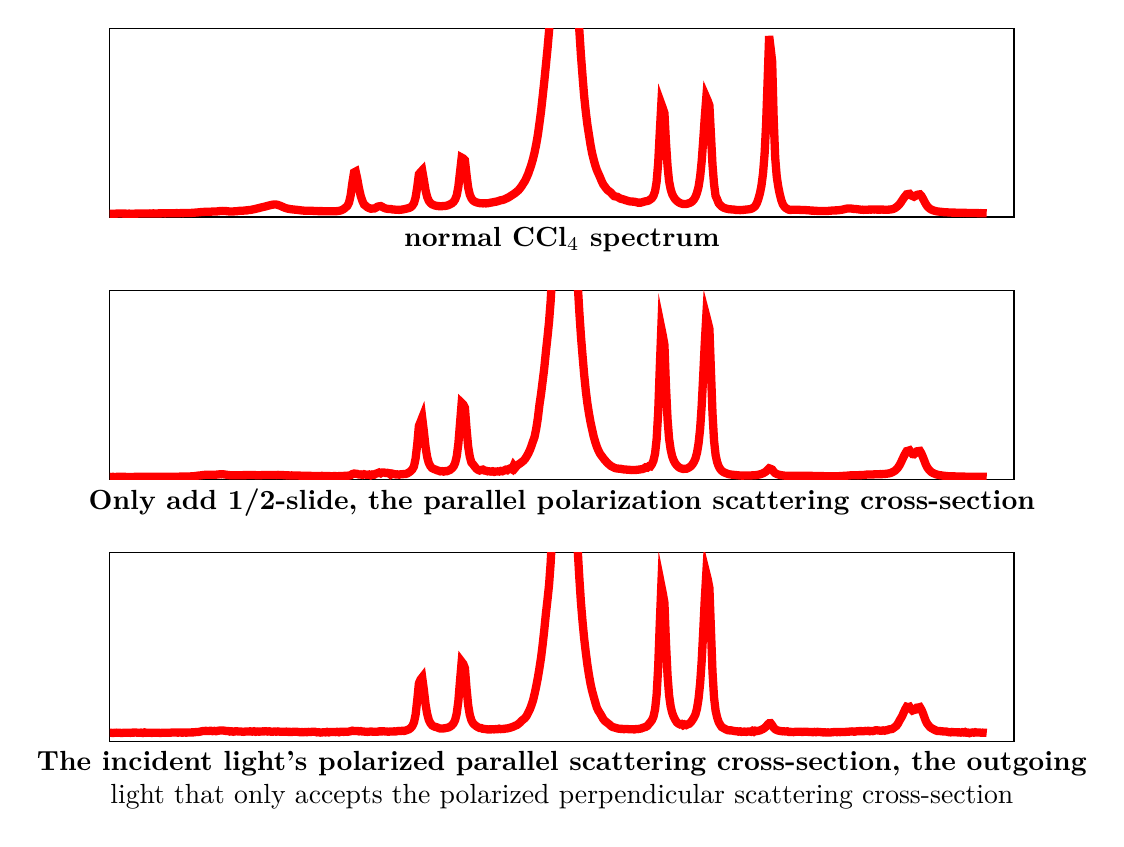
\begin{tikzpicture}

\begin{axis}[%
width=4.521in,
height=0.944in,
at={(0.758in,3.103in)},
scale only axis,
xmin=-1000,
xmax=1000,
xtick={\empty},
ymin=0,
ymax=180000,
ytick={\empty},
% axis background/.style={fill=white},
% title style={font=\bfseries},
% title={正常 CCl4 谱线},
xlabel={\bfseries normal CCl$_4$ spectrum},
xlabel style={yshift=0em},
xmajorgrids,
ymajorgrids
]
\addplot [color=red, line width=3.0pt, forget plot]
  table[row sep=crcr]{%
-1044.3	3066\\
-1040.3	3038.5\\
-1036.4	3043.1\\
-1032.5	2979.8\\
-1028.5	3007.5\\
-1024.6	2972\\
-1020.7	3026.5\\
-1016.8	3032.2\\
-1012.8	3108.1\\
-1008.9	3128\\
-1005	3139.9\\
-1001.1	3115.6\\
-997.1	3070\\
-993.2	3111.3\\
-989.3	3157.5\\
-985.4	3246.6\\
-981.5	3282.1\\
-977.6	3337\\
-973.7	3309.6\\
-969.8	3223.1\\
-965.9	3252\\
-961.9	3198.5\\
-958	3224.4\\
-954.1	3217\\
-950.2	3190.6\\
-946.3	3190\\
-942.4	3264.5\\
-938.6	3248.7\\
-934.7	3307.3\\
-930.8	3317\\
-926.9	3308.5\\
-923	3388.8\\
-919.1	3340\\
-915.2	3398\\
-911.3	3465.6\\
-907.4	3360.5\\
-903.6	3494.4\\
-899.7	3411\\
-895.8	3332\\
-891.9	3502.5\\
-888	3487.1\\
-884.2	3516.9\\
-880.3	3510\\
-876.4	3501.4\\
-872.6	3571.9\\
-868.7	3615.1\\
-864.8	3569.5\\
-861	3672.2\\
-857.1	3619\\
-853.2	3723.4\\
-849.4	3690.5\\
-845.5	3671.5\\
-841.7	3823.5\\
-837.8	3685.5\\
-833.9	3871\\
-830.1	3818.9\\
-826.2	3894.5\\
-822.4	3900.7\\
-818.5	3957.4\\
-814.7	4052\\
-810.9	4211.8\\
-807	4346.4\\
-803.2	4496.8\\
-799.3	4659.4\\
-795.5	4800.1\\
-791.6	4903.1\\
-787.8	5012.4\\
-784	5017\\
-780.1	5103\\
-776.3	5100.9\\
-772.5	5209.6\\
-768.7	5269.8\\
-764.8	5301.8\\
-761	5418.4\\
-757.2	5663.8\\
-753.3	5695.5\\
-749.5	5833.8\\
-745.7	5755\\
-741.9	5626.2\\
-738.1	5429\\
-734.3	5264.2\\
-730.4	5349\\
-726.6	5362.2\\
-722.8	5446.5\\
-719	5553.7\\
-715.2	5784.5\\
-711.4	5985.2\\
-707.6	6037.6\\
-703.8	6090\\
-700	6313\\
-696.2	6345.5\\
-692.4	6664.5\\
-688.6	6747.9\\
-684.8	7130\\
-681	7435.2\\
-677.2	7788.7\\
-673.4	8214.4\\
-669.6	8580.1\\
-665.8	9047.6\\
-662	9462.4\\
-658.3	9819.6\\
-654.5	10158\\
-650.7	10688.6\\
-646.9	11104.1\\
-643.1	11479.5\\
-639.4	11806.5\\
-635.6	11930.5\\
-631.8	11919.9\\
-628	11551.9\\
-624.3	10959.4\\
-620.5	10328.7\\
-616.7	9549.4\\
-612.9	8862\\
-609.2	8334.5\\
-605.4	7937.1\\
-601.6	7596.6\\
-597.9	7344.1\\
-594.1	7245.5\\
-590.4	7023\\
-586.6	6873.4\\
-582.9	6663.1\\
-579.1	6503.1\\
-575.3	6244.7\\
-571.6	6114\\
-567.8	5957.6\\
-564.1	6020.5\\
-560.3	5929\\
-556.6	6029.8\\
-552.9	5931.9\\
-549.1	5837.2\\
-545.4	5669.5\\
-541.6	5715\\
-537.9	5587.5\\
-534.1	5638.3\\
-530.4	5609.4\\
-526.7	5591\\
-522.9	5523.1\\
-519.2	5436.9\\
-515.5	5467\\
-511.8	5490.2\\
-508	5485.5\\
-504.3	5544.5\\
-500.6	5514.7\\
-496.9	5647.9\\
-493.1	5881.9\\
-489.4	6227.2\\
-485.7	6855.8\\
-482	7793.4\\
-478.3	9080.8\\
-474.5	10654.6\\
-470.8	13692.2\\
-467.1	20677.1\\
-463.4	32515.9\\
-459.7	42466.8\\
-456	43326\\
-452.3	35970.9\\
-448.6	27089.1\\
-444.9	20177.9\\
-441.2	15322.1\\
-437.5	11856.3\\
-437.5	11856.3\\
-433.8	10686.8\\
-430.1	9325.8\\
-426.4	8561.8\\
-422.7	7986.7\\
-419	8039.5\\
-415.3	8049\\
-411.6	8799.8\\
-407.9	9829.9\\
-404.2	10201.5\\
-400.6	10412.4\\
-396.9	9617\\
-393.2	8718.1\\
-389.5	8133.8\\
-385.8	7832.3\\
-382.1	7622\\
-378.5	7645\\
-374.8	7261.5\\
-371.1	7210.2\\
-367.4	6891.3\\
-363.8	6899.5\\
-360.1	6821.4\\
-356.4	6960.4\\
-352.8	7127.5\\
-349.1	7463.3\\
-345.4	7824.7\\
-341.8	8225.5\\
-338.1	8615.9\\
-334.4	9342.6\\
-330.8	10757.1\\
-327.1	13244.3\\
-323.5	18671.4\\
-319.8	28764.5\\
-316.2	40823.8\\
-312.5	42788\\
-308.9	44419.6\\
-305.2	35195.8\\
-301.6	25760.8\\
-297.9	19127.5\\
-294.3	15433.7\\
-290.6	13350.7\\
-287	12120.1\\
-283.3	11391.8\\
-279.7	10894.8\\
-276.1	10580.9\\
-272.4	10391.8\\
-268.8	10353.9\\
-265.2	10366.8\\
-261.5	10489.2\\
-257.9	10600.1\\
-254.3	10873.8\\
-250.6	11414.4\\
-247	12153.1\\
-243.4	12982.7\\
-239.7	14360.9\\
-236.1	16678.2\\
-232.5	20711.7\\
-228.9	28950.8\\
-225.3	42540.7\\
-221.6	56640.9\\
-218	55782\\
-214.4	54147.7\\
-210.8	40035.8\\
-207.2	28054.1\\
-203.6	21318.1\\
-200	17791.2\\
-196.4	15823.7\\
-192.8	14688.5\\
-189.1	14045.7\\
-185.5	13598.6\\
-181.9	13251.5\\
-178.3	13098.4\\
-174.7	13023.2\\
-171.1	13064.5\\
-167.5	13015.8\\
-163.9	13154.1\\
-160.4	13398.1\\
-156.8	13738.9\\
-153.2	14025.5\\
-149.6	14357.1\\
-146	14602.6\\
-142.4	14984\\
-138.8	15491.9\\
-135.2	15957.8\\
-131.6	16221.8\\
-128.1	16683.6\\
-124.5	17357.2\\
-120.9	18107.5\\
-117.3	18907\\
-113.7	19892.2\\
-110.2	20873.3\\
-106.6	21871.4\\
-103	22983.7\\
-99.5	24244.1\\
-95.9	25593.1\\
-92.3	27468.3\\
-88.7	29539.3\\
-85.2	32024.1\\
-81.6	34384\\
-78.1	37523.5\\
-74.5	41118.3\\
-70.9	45554.8\\
-67.4	50043.6\\
-63.8	55443.8\\
-60.3	61669.7\\
-56.7	69362.7\\
-53.1	78327.5\\
-49.6	89167.9\\
-46	100914.4\\
-42.5	114749.2\\
-38.9	129048.8\\
-35.4	144376.4\\
-31.9	159670.4\\
-28.3	177388.7\\
-24.8	200044.7\\
-21.2	231276.2\\
-17.7	270001.8\\
-14.1	324948.9\\
-10.6	498829.4\\
-7.1	905324.1\\
-3.5	1394210\\
0	1473772.5\\
3.5	1565129.5\\
7.1	1546555.5\\
10.6	1652176.3\\
14.1	1508172.5\\
17.6	1403928.2\\
21.2	772814.1\\
24.7	359192.5\\
28.2	255249.4\\
31.7	235274.4\\
35.3	203099.6\\
38.8	177064.8\\
42.3	153732.9\\
45.8	134125.3\\
49.3	115462.6\\
52.9	100527.3\\
56.4	88226.7\\
59.9	78540.5\\
63.4	68911.8\\
66.9	60956.7\\
70.4	54765\\
73.9	49320.5\\
77.4	44783.4\\
80.9	41391.5\\
84.4	37998.6\\
87.9	34370.7\\
91.4	31180.9\\
94.9	29108.1\\
98.4	27033.7\\
101.9	25410.1\\
105.4	24352.5\\
108.9	23071.7\\
112.4	21221.1\\
115.9	19879.1\\
119.4	19534.6\\
122.9	19272.4\\
126.3	18320\\
129.8	17505.9\\
133.3	17108.8\\
136.8	16735.1\\
140.3	16148.5\\
143.8	15729.5\\
147.2	15245.6\\
150.7	14909.4\\
154.2	14717.2\\
157.7	14699.5\\
161.1	14499.6\\
164.6	14136.2\\
168.1	13723.9\\
171.6	13714.5\\
175	13742.7\\
178.5	14180.1\\
182	14686\\
185.4	15001.6\\
188.9	15254.8\\
192.3	15776.2\\
195.8	16824.6\\
199.3	17981.7\\
202.7	20262.4\\
206.2	24624.7\\
209.6	33567.6\\
213.1	51591.1\\
216.5	79919\\
220	107725\\
223.4	103672.5\\
226.9	99230.1\\
230.3	71230.1\\
233.8	48377.2\\
237.2	34101.2\\
240.7	26453.1\\
244.1	21735.8\\
247.6	18980.7\\
251	16796.4\\
254.4	15321.6\\
257.9	14199.4\\
261.3	13350.7\\
264.7	12824.4\\
268.2	12479.7\\
271.6	12380.4\\
275	12440.6\\
278.5	12798.1\\
281.9	13279.7\\
285.3	13970.2\\
288.8	15062.9\\
292.2	16785.3\\
295.6	19242.6\\
299	23219.3\\
302.4	28875.7\\
305.9	38616\\
309.3	53089.5\\
312.7	73181.7\\
316.1	95029.5\\
319.5	113951.6\\
322.9	110599.5\\
326.4	106289.9\\
329.8	78160.5\\
333.2	49899\\
336.6	31507.3\\
340	20192.2\\
340	20192.2\\
343.4	16956.5\\
346.8	13279.4\\
350.2	11449.7\\
353.6	10081.4\\
357	9122.1\\
360.4	8491.2\\
363.8	8067.3\\
367.2	7697.8\\
370.6	7391.1\\
374	7317\\
377.4	7174.5\\
380.8	7059.8\\
384.2	6815.5\\
387.6	6779.3\\
391	6675.5\\
394.3	6588\\
397.7	6638.8\\
401.1	6799\\
404.5	6981.2\\
407.9	7122.9\\
411.3	7272.3\\
414.6	7433.5\\
418	7729.9\\
421.4	8339.1\\
424.8	9341.4\\
428.1	10758\\
431.5	13349.2\\
434.9	17597.2\\
438.3	22870.7\\
441.6	30193.1\\
445	41586.5\\
448.4	59858.1\\
451.7	87632\\
455.1	129593.9\\
458.5	172555.5\\
461.8	161055\\
465.2	148186.8\\
468.5	94378.8\\
471.9	56473.6\\
475.3	38643\\
478.6	29131.3\\
482	21780.1\\
485.3	16225.3\\
488.7	12190.2\\
492	10027\\
495.4	8600.8\\
498.7	7741.9\\
502.1	6973.8\\
505.4	6754.3\\
508.8	6875.5\\
512.1	6875.4\\
515.5	7001.5\\
518.8	6977.5\\
522.1	6892.1\\
525.5	6872\\
528.8	6679.5\\
532.2	6744.6\\
535.5	6629.3\\
538.8	6692.5\\
542.2	6464.5\\
545.5	6462\\
548.8	6256.3\\
552.1	6085.2\\
555.5	6137.5\\
558.8	5889.5\\
562.1	5961.6\\
565.5	5782\\
568.8	5806.5\\
572.1	5783.5\\
575.4	5728\\
578.7	5794\\
582.1	5705.7\\
585.4	5785.9\\
588.7	5808.1\\
592	5978.4\\
595.3	6051.3\\
598.6	6227.4\\
601.9	6150.5\\
605.3	6350.5\\
608.6	6365.3\\
611.9	6491.9\\
615.2	6693.1\\
618.5	6876.3\\
621.8	7189.9\\
625.1	7511.1\\
628.4	7906.6\\
631.7	8102.5\\
635	8124\\
638.3	8129.8\\
641.6	7994\\
644.9	7763.1\\
648.2	7651.5\\
651.5	7551.5\\
654.8	7394.3\\
658	7186.9\\
661.3	7007.3\\
664.6	7036.5\\
667.9	6834.9\\
671.2	6968\\
674.5	6888.8\\
677.8	7039.7\\
681.1	7104\\
684.3	7043.5\\
687.6	7154\\
690.9	7066.3\\
694.2	7126.4\\
697.4	7047.2\\
700.7	7045.5\\
704	7037.2\\
707.3	7095\\
710.5	7069.8\\
713.8	6984\\
717.1	6961\\
720.3	7010.3\\
723.6	7052.8\\
726.9	7220\\
730.1	7383.6\\
733.4	7814.8\\
736.7	8450.8\\
739.9	9461.3\\
743.2	10527.8\\
746.5	11999.7\\
749.7	13848.2\\
753	16063.3\\
756.2	18050.6\\
759.5	19963.2\\
762.7	21640.4\\
766	21925\\
769.2	22130.4\\
772.5	20568\\
775.7	20039.5\\
779	19389.7\\
782.2	20170.9\\
785.5	21107.5\\
788.7	21487.5\\
792	21644\\
795.2	20190.4\\
798.4	17772.9\\
801.7	15090.3\\
804.9	12493.7\\
808.1	10400.8\\
811.4	8882.5\\
814.6	7740.3\\
817.8	6988.9\\
821.1	6429.2\\
824.3	5991.3\\
827.5	5606\\
830.8	5321.4\\
834	5172.4\\
837.2	5046.5\\
840.4	4904.7\\
843.7	4709.6\\
846.9	4578.3\\
850.1	4491.4\\
853.3	4455.7\\
856.6	4334.6\\
859.8	4262.5\\
863	4204\\
866.2	4210\\
869.4	4197.5\\
872.6	4133\\
875.8	4086.6\\
879.1	4063\\
882.3	3968.8\\
885.5	4019.5\\
888.7	3953\\
891.9	4028\\
895.1	3923\\
898.3	3930.1\\
901.5	3771.5\\
904.7	3834.5\\
907.9	3821.2\\
911.1	3863.5\\
914.3	3801.3\\
917.5	3753.3\\
920.7	3724.8\\
923.9	3656.4\\
927.1	3716.2\\
930.3	3612\\
933.5	3657.7\\
936.7	3573.5\\
939.8	3564.7\\
};
\end{axis}

\begin{axis}[%
width=4.521in,
height=0.944in,
at={(0.758in,1.792in)},
scale only axis,
xmin=-1000,
xmax=1000,
xtick={\empty},
ymin=0,
ymax=120000,
ytick={\empty},
% axis background/.style={fill=white},
% title style={font=\bfseries},
% title={只加入 1/2 玻片, 偏振平行散射截面},
xlabel={\bfseries Only add 1/2-slide, the parallel polarization scattering cross-section},
xlabel style={yshift=0em},
xmajorgrids,
ymajorgrids
]
\addplot [color=red, line width=3.0pt, forget plot]
  table[row sep=crcr]{%
-1044.3	1476.9\\
-1040.3	1432\\
-1036.4	1416.1\\
-1032.5	1441.4\\
-1028.5	1452.3\\
-1024.6	1472.7\\
-1020.7	1445.5\\
-1016.8	1441.5\\
-1012.8	1450\\
-1008.9	1472.6\\
-1005	1452.5\\
-1001.1	1527\\
-997.1	1434.5\\
-993.2	1519.5\\
-989.3	1433.5\\
-985.4	1482\\
-981.5	1478.5\\
-977.6	1498.5\\
-973.7	1546.5\\
-969.8	1515\\
-965.9	1491.5\\
-961.9	1448.7\\
-958	1413.2\\
-954.1	1415.1\\
-950.2	1471.1\\
-946.3	1478\\
-942.4	1543\\
-938.6	1497\\
-934.7	1532\\
-930.8	1528.5\\
-926.9	1539.2\\
-923	1499.5\\
-919.1	1565.5\\
-915.2	1517.7\\
-911.3	1550.5\\
-907.4	1557.1\\
-903.6	1556\\
-899.7	1571.6\\
-895.8	1514\\
-891.9	1503.4\\
-888	1486.2\\
-884.2	1548.4\\
-880.3	1597.4\\
-876.4	1577\\
-872.6	1604.2\\
-868.7	1570.2\\
-864.8	1609.5\\
-861	1596.7\\
-857.1	1600.5\\
-853.2	1625\\
-849.4	1614.7\\
-845.5	1643.4\\
-841.7	1674.9\\
-837.8	1696.9\\
-833.9	1713.5\\
-830.1	1706.6\\
-826.2	1720.9\\
-822.4	1770.7\\
-818.5	1843.7\\
-814.7	1902.5\\
-810.9	2040.3\\
-807	2193.5\\
-803.2	2332.9\\
-799.3	2433.8\\
-795.5	2596.3\\
-791.6	2722\\
-787.8	2819.3\\
-784	2867.6\\
-780.1	2877.5\\
-776.3	2839.5\\
-772.5	2833.5\\
-768.7	2823.5\\
-764.8	2890.3\\
-761	2988.8\\
-757.2	3118\\
-753.3	3094\\
-749.5	3150.7\\
-745.7	3005.2\\
-741.9	2868.2\\
-738.1	2696\\
-734.3	2568.6\\
-730.4	2525\\
-726.6	2487.5\\
-722.8	2485.5\\
-719	2522.9\\
-715.2	2519.5\\
-711.4	2565.4\\
-707.6	2571.5\\
-703.8	2610\\
-700	2593\\
-696.2	2650.6\\
-692.4	2628.8\\
-688.6	2700.5\\
-684.8	2628\\
-681	2662.6\\
-677.2	2592.4\\
-673.4	2559.5\\
-669.6	2573.5\\
-665.8	2582.6\\
-662	2635.1\\
-658.3	2700.1\\
-654.5	2648\\
-650.7	2688.9\\
-646.9	2668\\
-643.1	2681\\
-639.4	2651.6\\
-635.6	2734.6\\
-631.8	2630\\
-628	2755.3\\
-624.3	2635.2\\
-620.5	2671\\
-616.7	2620.3\\
-612.9	2559.9\\
-609.2	2447.7\\
-605.4	2472\\
-601.6	2409\\
-597.9	2434.8\\
-594.1	2422.5\\
-590.4	2380\\
-586.6	2350.9\\
-582.9	2311.2\\
-579.1	2286.5\\
-575.3	2221\\
-571.6	2163.7\\
-567.8	2148.5\\
-564.1	2158.7\\
-560.3	2129\\
-556.6	2180\\
-552.9	2058.5\\
-549.1	2104\\
-545.4	2018.3\\
-541.6	2102.5\\
-537.9	2110.2\\
-534.1	2096\\
-530.4	2130\\
-526.7	2055.8\\
-522.9	2083.3\\
-519.2	2065.4\\
-515.5	2011.8\\
-511.8	1950.1\\
-508	1925.3\\
-504.3	1984.5\\
-500.6	1971\\
-496.9	1925.9\\
-493.1	1974.3\\
-489.4	2057.2\\
-485.7	2101.1\\
-482	2114.1\\
-478.3	2182.3\\
-474.5	2261.5\\
-470.8	2299.1\\
-467.1	2538.2\\
-463.4	3284.7\\
-463.4	3284.7\\
-459.7	3596.9\\
-456	3514\\
-452.3	3379.8\\
-448.6	2997\\
-444.9	3068.9\\
-441.2	2739.5\\
-437.5	3180\\
-433.8	2914.3\\
-430.1	2833.7\\
-426.4	3014.5\\
-422.7	2481\\
-419	3034.5\\
-415.3	2865.2\\
-411.6	3496.7\\
-407.9	3791.9\\
-404.2	4255\\
-400.6	3734.5\\
-396.9	4290\\
-393.2	4281.9\\
-389.5	3961\\
-385.8	4041.9\\
-382.1	3830.5\\
-378.5	2912\\
-374.8	3534\\
-371.1	3247.6\\
-367.4	3042.5\\
-363.8	3094\\
-360.1	2906.8\\
-356.4	3174.1\\
-352.8	3193.3\\
-349.1	3310\\
-345.4	3352.2\\
-341.8	3725.9\\
-338.1	4315.4\\
-334.4	5127.4\\
-330.8	6220.4\\
-327.1	8138.6\\
-323.5	13186.8\\
-319.8	22378.6\\
-316.2	33883.1\\
-312.5	36513.5\\
-308.9	39127.5\\
-305.2	30401.2\\
-301.6	20792.4\\
-297.9	14118.2\\
-294.3	10316.7\\
-290.6	8257.4\\
-287	7063\\
-283.3	6517.2\\
-279.7	6165.1\\
-276.1	5676.3\\
-272.4	5393.1\\
-268.8	5003\\
-265.2	5145.5\\
-261.5	4853.8\\
-257.9	5151\\
-254.3	5109.1\\
-250.6	5500.1\\
-247	5999.6\\
-243.4	6881.7\\
-239.7	8010.9\\
-236.1	10205.9\\
-232.5	14548.5\\
-228.9	22526.6\\
-225.3	35363.8\\
-221.6	48491.4\\
-218	47487.5\\
-214.4	45415.8\\
-210.8	32086.8\\
-207.2	20701.3\\
-203.6	14266.4\\
-200	10587.1\\
-196.4	9442.8\\
-192.8	8035.9\\
-189.1	6765.2\\
-185.5	5972\\
-181.9	5556.2\\
-178.3	5932.5\\
-174.7	6126.2\\
-171.1	5525.5\\
-167.5	5368.8\\
-163.9	5005.5\\
-160.4	5016.6\\
-156.8	4844.3\\
-153.2	5066\\
-149.6	4655.4\\
-146	4908.5\\
-142.4	4982.4\\
-138.8	4871.5\\
-135.2	5274\\
-131.6	5067.8\\
-128.1	5515\\
-124.5	6020.3\\
-120.9	5724\\
-117.3	6533\\
-113.7	6956.1\\
-110.2	6334.5\\
-106.6	8640\\
-103	7326.9\\
-99.5	8554.4\\
-95.9	9371.9\\
-92.3	10087.6\\
-88.7	10853.7\\
-85.2	11683.8\\
-81.6	12780.8\\
-78.1	14381.5\\
-74.5	16221.3\\
-70.9	18404.4\\
-67.4	20985\\
-63.8	24093.8\\
-60.3	26924.6\\
-56.7	32129.3\\
-53.1	38710.1\\
-49.6	47155.6\\
-46	54218.6\\
-42.5	62242.2\\
-38.9	70609.3\\
-35.4	80703.9\\
-31.9	89905.8\\
-28.3	100121.8\\
-24.8	113032.9\\
-21.2	131422.4\\
-17.7	153388\\
-14.1	184421.1\\
-10.6	250157\\
-7.1	479118.9\\
-3.5	892697.1\\
0	1338776.8\\
3.5	1621396.7\\
7.1	1546301\\
10.6	1538865.4\\
14.1	1204997.2\\
17.6	741571.8\\
21.2	326084.5\\
24.7	180010.9\\
28.2	159306.7\\
31.7	142039\\
35.3	122892.4\\
38.8	105683.4\\
42.3	90763.9\\
45.8	78434.6\\
49.3	66696.4\\
52.9	56437.9\\
56.4	48294.2\\
59.9	41916.4\\
63.4	36263\\
66.9	31657.1\\
70.4	27136.2\\
73.9	23671.6\\
77.4	20588.3\\
80.9	18226.6\\
84.4	16241.8\\
87.9	14870.9\\
91.4	13497.7\\
94.9	12208.6\\
98.4	11107.1\\
101.9	10044.3\\
105.4	9158.7\\
108.9	8363.9\\
112.4	7866.2\\
115.9	7331.1\\
119.4	6938.1\\
122.9	6793.5\\
126.3	6698\\
129.8	6637.5\\
133.3	6416.9\\
136.8	6242.1\\
140.3	6200.8\\
143.8	6086.3\\
147.2	6056\\
150.7	5931.2\\
154.2	5808.8\\
157.7	5867\\
161.1	5847.5\\
164.6	5934.7\\
168.1	6004.5\\
171.6	6179\\
175	6326.5\\
178.5	6485.1\\
182	6856\\
185.4	7563.5\\
188.9	7383\\
192.3	8214.5\\
195.8	8109.4\\
199.3	9581\\
202.7	11915.3\\
206.2	16352.3\\
209.6	25259.2\\
213.1	42664.4\\
216.5	69949.1\\
220	95972.4\\
223.4	91147\\
226.9	85441.4\\
230.3	58906.4\\
233.8	38114.5\\
237.2	25726.8\\
240.7	18776.5\\
244.1	14486.4\\
247.6	11813.5\\
251	10043.3\\
254.4	8764.9\\
257.9	7810.1\\
261.3	7186.3\\
264.7	6822.6\\
268.2	6565.7\\
271.6	6607.5\\
275	6601.5\\
278.5	7019.3\\
281.9	7543.1\\
285.3	8264\\
288.8	9417.9\\
292.2	10989.9\\
295.6	13220\\
299	16911.3\\
302.4	22709.8\\
305.9	32157.5\\
309.3	46739\\
312.7	65962.8\\
316.1	86370.1\\
319.5	103581.8\\
322.9	99832.5\\
326.4	95617.3\\
329.8	68580.4\\
333.2	42019\\
336.6	24626.8\\
340	15562.6\\
343.4	10954.2\\
346.8	8256.2\\
350.2	6525.6\\
353.6	5384.3\\
357	4660.7\\
360.4	4148.5\\
363.8	3787.1\\
367.2	3404.8\\
370.6	3144.7\\
374	2985.2\\
377.4	2852.6\\
380.8	2763.7\\
384.2	2649.6\\
387.6	2558.4\\
391	2464.1\\
394.3	2369\\
397.7	2292.7\\
401.1	2276.7\\
404.5	2360\\
407.9	2339\\
411.3	2342.7\\
414.6	2324\\
418	2379.2\\
421.4	2484.6\\
424.8	2529.5\\
428.1	2575.5\\
431.5	2655.8\\
434.9	2903.1\\
438.3	3120.5\\
441.6	3438.9\\
445	3796.7\\
448.4	4314.6\\
451.7	4938.7\\
455.1	5962\\
458.5	6928.1\\
461.8	6607\\
465.2	6149\\
468.5	4837.2\\
471.9	3830.7\\
475.3	3340.4\\
478.6	3015\\
482	2775.6\\
485.3	2565.3\\
488.7	2439\\
492	2292.4\\
495.4	2187.3\\
498.7	2189.7\\
502.1	2120\\
505.4	2194.5\\
508.8	2127.9\\
512.1	2159\\
515.5	2157.4\\
518.8	2215.5\\
522.1	2217.9\\
525.5	2239.8\\
528.8	2189.6\\
532.2	2184.5\\
535.5	2210.9\\
538.8	2204\\
542.2	2217.4\\
545.5	2241.5\\
548.8	2148\\
552.1	2154.7\\
555.5	2082.2\\
558.8	2044.6\\
562.1	2047\\
565.5	2006.2\\
568.8	2019.5\\
572.1	2028\\
575.4	1992.7\\
578.7	1964.7\\
582.1	1899.8\\
585.4	1927.5\\
588.7	1875.6\\
592	1891.4\\
595.3	1885.9\\
598.6	1913.3\\
601.9	1918.1\\
605.3	1934.5\\
608.6	1943.2\\
611.9	1938.1\\
615.2	1989.4\\
618.5	2032.5\\
621.8	2114\\
625.1	2122.1\\
628.4	2253.2\\
631.7	2278\\
635	2382.2\\
638.3	2457.6\\
641.6	2525\\
644.9	2496.5\\
648.2	2485.5\\
651.5	2535.7\\
654.8	2473\\
658	2627.5\\
661.3	2577\\
664.6	2667\\
667.9	2734.7\\
671.2	2844.5\\
674.5	2960.7\\
677.8	3033.6\\
681.1	3019.1\\
684.3	3062\\
687.6	3022.6\\
690.9	3097.2\\
694.2	3111.6\\
697.4	3167.1\\
700.7	3154.5\\
704	3241.8\\
707.3	3192.5\\
710.5	3326\\
713.8	3320.8\\
717.1	3459.2\\
720.3	3574.9\\
723.6	3703.7\\
726.9	3967.9\\
730.1	4315.4\\
733.4	4815.8\\
736.7	5392\\
739.9	6232.7\\
743.2	7236.7\\
746.5	8699.5\\
749.7	10444\\
753	12471.7\\
756.2	14440.2\\
759.5	16287.9\\
762.7	17850.3\\
766	18054\\
769.2	18373.8\\
772.5	17047.2\\
775.7	15957.1\\
779	15852.4\\
782.2	16666.2\\
785.5	17724.7\\
788.7	17860\\
792	17992.7\\
795.2	16469.6\\
798.4	14261.4\\
801.7	11890.5\\
804.9	9454.7\\
808.1	7613.8\\
811.4	6237.2\\
814.6	5251.9\\
817.8	4439.5\\
821.1	3922.8\\
824.3	3511.6\\
827.5	3175.7\\
830.8	2887.8\\
834	2693.4\\
837.2	2522.1\\
840.4	2414.2\\
843.7	2232.6\\
846.9	2158.6\\
850.1	2029.6\\
853.3	1971.2\\
856.6	1905.4\\
859.8	1932.9\\
863	1887\\
866.2	1815.8\\
869.4	1817.5\\
872.6	1733.3\\
875.8	1780\\
879.1	1707.4\\
882.3	1730.5\\
885.5	1704\\
888.7	1637\\
891.9	1636.5\\
895.1	1606.5\\
898.3	1598.2\\
901.5	1622\\
904.7	1608.5\\
907.9	1633.9\\
911.1	1612.6\\
914.3	1625.5\\
917.5	1600.9\\
920.7	1571.3\\
923.9	1560.5\\
927.1	1600.5\\
930.3	1612\\
933.5	1615.7\\
936.7	1621.7\\
939.8	1589\\
};
\end{axis}

\begin{axis}[%
width=4.521in,
height=0.944in,
at={(0.758in,0.481in)},
scale only axis,
xmin=-1000,
xmax=1000,
xtick={\empty},
ymin=0,
ymax=26000,
ytick={\empty},
% axis background/.style={fill=white},
% title style={font=\bfseries},
% title={入射光偏振平行散射截面, 只接受偏振垂直散射截面的出射光},
xlabel={
    \shortstack{
        \bfseries
        The incident light's polarized parallel scattering cross-section, the outgoing
        \\
        light that only accepts the polarized perpendicular scattering cross-section
    }
},
xlabel style={yshift=0em},
xmajorgrids,
ymajorgrids
]
\addplot [color=red, line width=3.0pt, forget plot]
  table[row sep=crcr]{%
-1044.3	1132.3\\
-1040.3	1172\\
-1036.4	1156.6\\
-1032.5	1187.5\\
-1028.5	1187.6\\
-1024.6	1188\\
-1020.7	1205\\
-1016.8	1179.5\\
-1012.8	1186.9\\
-1008.9	1177\\
-1005	1207\\
-1001.1	1175.2\\
-997.1	1194\\
-993.2	1160.9\\
-989.3	1188.1\\
-985.4	1208.1\\
-981.5	1191.1\\
-977.6	1197\\
-973.7	1156.5\\
-969.8	1187.3\\
-965.9	1200.5\\
-961.9	1192.1\\
-958	1189.5\\
-954.1	1178.3\\
-950.2	1209.5\\
-946.3	1210.5\\
-942.4	1230\\
-938.6	1191.5\\
-934.7	1189.2\\
-930.8	1215\\
-926.9	1160\\
-923	1244.5\\
-919.1	1184.5\\
-915.2	1204.9\\
-911.3	1201.5\\
-907.4	1171.5\\
-903.6	1190.4\\
-899.7	1187.2\\
-895.8	1182.7\\
-891.9	1193\\
-888	1159.4\\
-884.2	1197\\
-880.3	1183\\
-876.4	1199.7\\
-872.6	1190.5\\
-868.7	1182.4\\
-864.8	1207.2\\
-861	1232.1\\
-857.1	1223.8\\
-853.2	1228.5\\
-849.4	1205.8\\
-845.5	1227.8\\
-841.7	1212.5\\
-837.8	1213.7\\
-833.9	1219\\
-830.1	1206.5\\
-826.2	1236.6\\
-822.4	1218.5\\
-818.5	1248.5\\
-814.7	1247\\
-810.9	1280\\
-807	1294\\
-803.2	1311.4\\
-799.3	1358.6\\
-795.5	1417.3\\
-791.6	1437.1\\
-787.8	1456\\
-784	1439.4\\
-780.1	1446.5\\
-776.3	1465.8\\
-772.5	1415.5\\
-768.7	1452.1\\
-764.8	1404.2\\
-761	1461.9\\
-757.2	1494.3\\
-753.3	1508.6\\
-749.5	1506.5\\
-745.7	1469.5\\
-741.9	1438.2\\
-738.1	1441.5\\
-734.3	1361.5\\
-730.4	1400.5\\
-726.6	1333.8\\
-722.8	1384.5\\
-719	1390.6\\
-715.2	1377\\
-711.4	1369.5\\
-707.6	1346.5\\
-703.8	1321\\
-700	1365\\
-696.2	1366.4\\
-692.4	1379.1\\
-688.6	1384\\
-684.8	1346.6\\
-681	1402\\
-677.2	1327.5\\
-673.4	1373\\
-669.6	1340.8\\
-665.8	1362.5\\
-662	1383.5\\
-658.3	1378\\
-654.5	1407.5\\
-650.7	1355.5\\
-646.9	1396.5\\
-643.1	1336.5\\
-639.4	1341.3\\
-635.6	1369.2\\
-631.8	1335\\
-628	1378.1\\
-624.3	1341.9\\
-620.5	1340.3\\
-616.7	1344.5\\
-612.9	1332.5\\
-609.2	1350.6\\
-605.4	1316\\
-601.6	1319.1\\
-597.9	1295.9\\
-594.1	1332.5\\
-590.4	1320\\
-586.6	1335.3\\
-582.9	1304.9\\
-579.1	1268.7\\
-575.3	1287.5\\
-571.6	1266\\
-567.8	1299\\
-564.1	1266.5\\
-560.3	1310.5\\
-556.6	1289\\
-552.9	1327.9\\
-549.1	1324.3\\
-545.4	1315\\
-541.6	1249.9\\
-537.9	1273.5\\
-534.1	1216.5\\
-530.4	1241.4\\
-526.7	1267\\
-522.9	1246\\
-519.2	1314.5\\
-515.5	1243\\
-511.8	1302\\
-508	1286.1\\
-504.3	1304\\
-500.6	1285.6\\
-496.9	1327\\
-493.1	1261.5\\
-489.4	1337.5\\
-485.7	1321.5\\
-482	1317\\
-478.3	1326\\
-474.5	1319.3\\
-470.8	1359.5\\
-467.1	1407.8\\
-463.4	1476.4\\
-459.7	1439.5\\
-456	1439.6\\
-452.3	1446.5\\
-448.6	1385\\
-444.9	1427.3\\
-441.2	1362\\
-437.5	1353.2\\
-433.8	1336.5\\
-430.1	1312.6\\
-426.4	1339.8\\
-422.7	1365.4\\
-419	1346.1\\
-415.3	1333.5\\
-411.6	1323.6\\
-407.9	1333\\
-404.2	1382.5\\
-400.6	1383\\
-396.9	1384.3\\
-393.2	1391.6\\
-389.5	1359.7\\
-385.8	1351\\
-382.1	1342.3\\
-378.5	1373.1\\
-374.8	1371.5\\
-371.1	1386\\
-367.4	1374.6\\
-363.8	1420.2\\
-360.1	1448.3\\
-356.4	1433.4\\
-352.8	1471\\
-349.1	1444.4\\
-345.4	1500.2\\
-341.8	1581\\
-338.1	1671\\
-334.4	1844.9\\
-330.8	2109.7\\
-327.1	2614.9\\
-323.5	3672.8\\
-319.8	5714.5\\
-316.2	8009.2\\
-312.5	8522\\
-308.9	8809\\
-305.2	7094.7\\
-301.6	5172.4\\
-297.9	3802.9\\
-294.3	2961.6\\
-290.6	2503.9\\
-287	2212\\
-283.3	2074.9\\
-279.7	1995.6\\
-276.1	1944.4\\
-272.4	1841.8\\
-268.8	1771.5\\
-265.2	1771\\
-261.5	1791.8\\
-257.9	1827.9\\
-254.3	1871\\
-250.6	1924.8\\
-247	2046.6\\
-243.4	2211.8\\
-239.7	2478.7\\
-236.1	2939.7\\
-232.5	3857.2\\
-228.9	5569.7\\
-225.3	8313.3\\
-221.6	10973.2\\
-218	10680\\
-214.4	10092.2\\
-210.8	7295.9\\
-207.2	4995.5\\
-203.6	3655\\
-200	2899.3\\
-196.4	2502.1\\
-192.8	2283\\
-189.1	2095\\
-185.5	1959.2\\
-181.9	1847.3\\
-178.3	1834\\
-174.7	1736\\
-171.1	1723\\
-167.5	1688.5\\
-163.9	1645.3\\
-160.4	1663.6\\
-156.8	1660\\
-153.2	1666.5\\
-149.6	1659.4\\
-146	1697.1\\
-142.4	1678\\
-138.8	1754.5\\
-135.2	1693\\
-131.6	1723.7\\
-128.1	1726.5\\
-124.5	1764.9\\
-120.9	1785.2\\
-117.3	1844.4\\
-113.7	1895\\
-110.2	1979.5\\
-106.6	2051.5\\
-103	2165.4\\
-99.5	2253.2\\
-95.9	2422.8\\
-92.3	2602.2\\
-88.7	2856.5\\
-85.2	3022.3\\
-81.6	3223.9\\
-78.1	3496.4\\
-74.5	3948.7\\
-70.9	4395.6\\
-67.4	4954.5\\
-63.8	5632.5\\
-60.3	6545.1\\
-56.7	7591\\
-53.1	8758.2\\
-49.6	10079.8\\
-46	11542.2\\
-42.5	13298.6\\
-38.9	15334.3\\
-35.4	17529.1\\
-31.9	19436.9\\
-28.3	21559.4\\
-24.8	24539.2\\
-21.2	28736.6\\
-17.7	33460.5\\
-14.1	40235.5\\
-10.6	53661.7\\
-7.1	104039.1\\
-3.5	284349.1\\
0	612437.4\\
3.5	897396.5\\
7.1	882734.9\\
10.6	590069.7\\
14.1	275444.8\\
17.6	106448.9\\
21.2	54439.7\\
24.7	40349.2\\
28.2	35329.8\\
31.7	30596.8\\
35.3	26138.8\\
38.8	22386\\
42.3	19075.4\\
45.8	16485.1\\
49.3	14207\\
52.9	12278.1\\
56.4	10592.9\\
59.9	9178.1\\
63.4	7949.1\\
66.9	6967.1\\
70.4	6171.1\\
73.9	5391.8\\
77.4	4668.2\\
80.9	4209.6\\
84.4	3878.6\\
87.9	3501.7\\
91.4	3104.1\\
94.9	2831.8\\
98.4	2665.6\\
101.9	2493.7\\
105.4	2319.8\\
108.9	2121\\
112.4	1981.1\\
115.9	1923.1\\
119.4	1862\\
122.9	1794.1\\
126.3	1747\\
129.8	1728.8\\
133.3	1728.5\\
136.8	1690.5\\
140.3	1701.5\\
143.8	1710.3\\
147.2	1689\\
150.7	1678\\
154.2	1670.5\\
157.7	1662.9\\
161.1	1659.3\\
164.6	1709.5\\
168.1	1698.2\\
171.6	1747\\
175	1774.4\\
178.5	1867.3\\
182	1935.6\\
185.4	1997.4\\
188.9	2130.2\\
192.3	2379\\
195.8	2636.3\\
199.3	2934.7\\
202.7	3416.6\\
206.2	4419.6\\
209.6	6388.5\\
213.1	10279.7\\
216.5	16070\\
220	21429.8\\
223.4	20361\\
226.9	19089.4\\
230.3	13555.4\\
233.8	9046\\
237.2	6360.2\\
240.7	4807.8\\
244.1	3941.3\\
247.6	3354.8\\
251	2952.6\\
254.4	2630.3\\
257.9	2450.6\\
261.3	2342\\
264.7	2396\\
268.2	2224.5\\
271.6	2338.5\\
275	2250.9\\
278.5	2369.6\\
281.9	2435.7\\
285.3	2641\\
288.8	2948.7\\
292.2	3289.6\\
295.6	3736.5\\
299	4549.8\\
302.4	5885.8\\
305.9	8010.6\\
309.3	11072.6\\
312.7	15163.8\\
316.1	19537.9\\
319.5	23131.2\\
322.9	22277.5\\
326.4	21132.9\\
329.8	15344.7\\
333.2	9597.6\\
336.6	6053.5\\
340	4259.8\\
343.4	3330.8\\
346.8	2692.4\\
350.2	2291.7\\
353.6	1987.1\\
357	1857.7\\
360.4	1743.2\\
363.8	1627.7\\
367.2	1545.4\\
370.6	1521.2\\
374	1528.7\\
377.4	1483.4\\
380.8	1440.3\\
384.2	1409.4\\
387.6	1413.3\\
391	1343.6\\
394.3	1391\\
397.7	1317.5\\
401.1	1344.4\\
404.5	1351\\
407.9	1314\\
411.3	1358\\
414.6	1364.7\\
418	1332\\
421.4	1456.5\\
424.8	1337.5\\
428.1	1474.5\\
431.5	1427.1\\
434.9	1470\\
438.3	1516.8\\
441.6	1616.2\\
445	1714.6\\
448.4	1856.4\\
451.7	2042\\
455.1	2304.8\\
458.5	2504.6\\
461.8	2515.4\\
465.2	2238.7\\
468.5	1899.6\\
471.9	1681.8\\
475.3	1561.8\\
478.6	1491.1\\
482	1446.9\\
485.3	1413.1\\
488.7	1385.9\\
492	1392.9\\
495.4	1360.9\\
498.7	1392\\
502.1	1305\\
505.4	1319.3\\
508.8	1305.5\\
512.1	1282.7\\
515.5	1314.9\\
518.8	1336\\
522.1	1337.5\\
525.5	1324.6\\
528.8	1334\\
532.2	1298\\
535.5	1337\\
538.8	1326.8\\
542.2	1334.8\\
545.5	1305.9\\
548.8	1291.5\\
552.1	1287.1\\
555.5	1273.6\\
558.8	1309.9\\
562.1	1271\\
565.5	1322.7\\
568.8	1295.4\\
572.1	1291.5\\
575.4	1257.8\\
578.7	1237.5\\
582.1	1259.4\\
585.4	1225.5\\
588.7	1249.2\\
592	1228.2\\
595.3	1244\\
598.6	1270.4\\
601.9	1288.6\\
605.3	1299.2\\
608.6	1271\\
611.9	1300.6\\
615.2	1277.5\\
618.5	1303.2\\
621.8	1292.5\\
625.1	1296.5\\
628.4	1317.5\\
631.7	1342\\
635	1345.4\\
638.3	1362.5\\
641.6	1381.8\\
644.9	1352.5\\
648.2	1345.8\\
651.5	1383\\
654.8	1405.8\\
658	1419.5\\
661.3	1421.2\\
664.6	1410\\
667.9	1410.2\\
671.2	1451.3\\
674.5	1437.8\\
677.8	1467.5\\
681.1	1403\\
684.3	1442.2\\
687.6	1420.1\\
690.9	1468.5\\
694.2	1534.2\\
697.4	1536.3\\
700.7	1495.4\\
704	1483.6\\
707.3	1477\\
710.5	1520\\
713.8	1473\\
717.1	1540.9\\
720.3	1559\\
723.6	1657.6\\
726.9	1690.3\\
730.1	1701.4\\
733.4	1830\\
736.7	1994.9\\
739.9	2144.3\\
743.2	2431.6\\
746.5	2826.2\\
749.7	3158.7\\
753	3526\\
756.2	3985\\
759.5	4427.3\\
762.7	4769.1\\
766	4705.5\\
769.2	4769.3\\
772.5	4466.4\\
775.7	4254\\
779	4333\\
782.2	4376.5\\
785.5	4653.9\\
788.7	4665.5\\
792	4725.5\\
795.2	4396.5\\
798.4	3933.5\\
801.7	3364.5\\
804.9	2831.1\\
808.1	2451.8\\
811.4	2186.4\\
814.6	1961.1\\
817.8	1816.5\\
821.1	1707.5\\
824.3	1606\\
827.5	1505\\
830.8	1437.5\\
834	1432.2\\
837.2	1417.6\\
840.4	1389.5\\
843.7	1380.2\\
846.9	1360\\
850.1	1371.1\\
853.3	1307.2\\
856.6	1272\\
859.8	1248.2\\
863	1304.7\\
866.2	1275.5\\
869.4	1274.9\\
872.6	1258.5\\
875.8	1241.5\\
879.1	1249\\
882.3	1213.4\\
885.5	1274.5\\
888.7	1230.8\\
891.9	1303.5\\
895.1	1208.5\\
898.3	1218.7\\
901.5	1140.3\\
904.7	1200\\
907.9	1238.7\\
911.1	1209.5\\
914.3	1271\\
917.5	1222.1\\
920.7	1232.6\\
923.9	1231.5\\
927.1	1194.6\\
930.3	1211\\
933.5	1204.8\\
936.7	1202\\
939.8	1183\\
};
\end{axis}
\end{tikzpicture}%}
% \end{figure}
This is related to the fact that the $A_1$ representation is the trivial representation. For an $A_1$ vibrational mode, the polarizability tensor $\overset{\leftrightarrow}{\boldsymbol{\alpha }}\sim \overset{\leftrightarrow}{\boldsymbol{I}}$, the latter being the identity tensor. In other words, whatever polarization state $\psi$ is incident, the scattered light must emerge in the same state $\psi$; any experimental configuration that cannot receive the polarization state $\psi$ will cause the $A_1$ peak to disappear.

This example inspires a more general observation: a necessary and sufficient condition for observing the disappearance of an $A_1$ peak in a polarization experiment on another substance is that the molecular vibrational modes include an $A_1$ representation---for example, $\ce{CO2}$.

\paragraph{Similarities among Isostructural Molecules}

Isostructural molecules will yield the same normal modes when analyzed by the method of Section~\ref{subsec}. For example, $\ce{CH4}$ will have the same modes as $\ce{CCl4}$. This does not, however, imply that the two spectra are similar: one must also consider the difference in first-order force constants between the two systems, which depends primarily on the masses of the atoms involved. Differing force constants will affect the magnitude of the Raman shifts and the signal intensities. Nevertheless, one can predict that $\ce{CH4}$ will also exhibit 4 Stokes peaks, and that one of them will disappear in a polarization experiment.


\end{document}